\chapter{ICE AGE OF CRYPTOCURRENCIES}
\label{ch:iceage}

As the mother of all things crypto, Bitcoin holds the lion's share in the total cryptocurrency market at the point of writing. \Cref{tab:historicalmarketcap} shows some key historical figures in terms of cryptocurrency market capitalisation. Please note the enormous volatility that haunts this market up until this day and the rapid increase of cryptocurrency and blockchain-based projects that make up this market. The total market cap, the volume traded over the last 24 hours, and the ratio of BTC dominance relative to total market capitalization are subject to market activity and dynamics. Hence these values are subject to change and only serve as a first insight into the cryptocurrency market development of the last few years based on only a few parameters.\medskip 


\begin{table}[ht]
\centering
\caption{Historical snapshots cryptocurrency market capitalisation}
\begin{tabular}{@{}lllllr@{}}

             \toprule
\textbf{Q} & \textbf{Date} & \textbf{Assets} & \textbf{Market cap.} & \textbf{24h vol.} & \textbf{BTC dom.} \\
\midrule
      
Q1       & 1-Jan-2015     & 533           & \$          5,483,191,815 & \$                 17,590,900 & 78.3\%  \\
Q2       & 1-Apr-2015     & 553           & \$          3,951,215,532 & \$                 26,496,700 & 87.5\%  \\
Q3       & 1-Jul-2015     & 588           & \$          4,450,571,456 & \$                 41,494,000 & 83.2\%  \\
Q4       & 1-Oct-2015     & 599           & \$          4,015,520,613 & \$                 23,581,000 & 86.5\%  \\
Q1       & 1-Jan-2016     & 573           & \$          7,135,452,840 & \$                 48,482,900 & 91.3\%  \\
Q2       & 1-Apr-2016     & 541           & \$          8,137,620,941 & \$                 80,037,900 & 78.8\%  \\
Q2       & 1-Jul-2016     & 608           & \$        12,788,684,228  & \$              170,788,000   & 83.0\%  \\
Q4       & 1-Oct-2016     & 650           & \$        12,228,772,789  & \$                 86,459,400 & 79.4\%  \\
Q1       & 1-Jan-2017     & 636           & \$        18,260,123,309  & \$              121,072,000   & 87.2\%  \\
Q2       & 1-Apr-2017     & 763           & \$        26,095,849,095  & \$              578,474,000   & 67.2\%  \\
Q3       & 1-Jul-2017     & 880           & \$        95,604,911,387  & \$           2,715,040,000    & 41.1\%  \\
Q4       & 1-Oct-2017     & 1111          & \$     148,853,058,782    & \$           2,520,660,000    & 48.8\%  \\
Q1       & 1-Jan-2018     & 1365          & \$     616,875,617,584    & \$        24,719,400,000      & 38.2\%  \\
Q2       & 1-Apr-2018     & 1557          & \$     254,298,972,658    & \$           9,942,170,000    & 45.4\% \\
Q3       & 1-Jul-2018     & 1573          & \$     257,373,095,796    & \$        13,875,600,000      & 42.6\% \\
Q4       & 1-Oct-2018     & 1925          & \$     222,182,499,719    & \$        15,176,969,795      & 51.7\% \\
Q1       & 1-Jan-2019     & 2076          & \$     129,940,274,883    & \$        13,463,554,390      & 51.6\% \\
Q2       & 1-Apr-2019     & 2138          & \$     170,879,300,093    & \$          45,035,593,451    & 54.4\%  \\
Q3       & 1-Jul-2019     & 2254          & \$     310,619,496,955    & \$           58,374,967,544   & 65.3\%  \\
Q4       & 1-Oct-2019     & N/A          & \$      221,235,513,684    & \$           61,555,937,344   & 65.3\% \\
Q1       & 1-Jan-2020     & 5154          & \$     191,542,043,659    & \$            66,156,212,697   & 68.3\% \\

\bottomrule
\end{tabular}
\label{tab:historicalmarketcap}
\source{Coinmarketcap, 27-02-2020; \textit{Historical Market Data.}}
\end{table}

\section{Volatility}
The global historical chart presented in  \cref{fig:totalmarketcap} shows an immense amount of volatility in cryptocurrency markets. As you can see, total market hovered around \$1-2B in 2013 and peaked right before 2014 up to \$10B, it then remained rather constant up to 2017 where things started moving after massive amounts of liquidity entered the market. It has since then peaked at just over \$800B in early 2018 and has been receding ever since, with the occasional upward movements over a relatively small time-span. Speculation and hype drove market capitalization through the roof in late 2017 and early 2018. Everybody was talking about cryptocurrency and blockchain in those days, but regular fear-mongering sentiment was much around, and people were very skeptical of the future of cryptocurrency.
 
    \begin{figure}[htb]
        \centering
        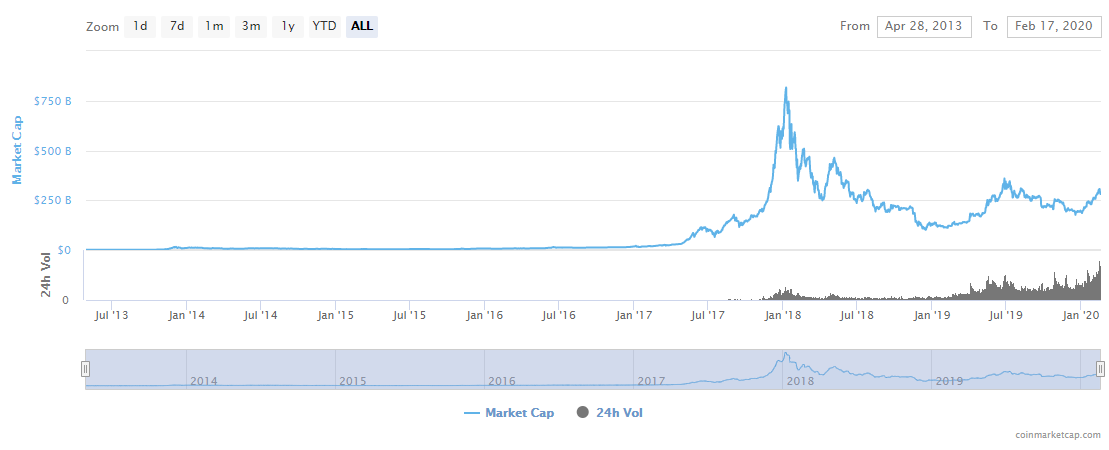
\includegraphics[width=\textwidth]{img/ch-iceage/cmc_mcapchart_feb2020.PNG}
        \caption{Global Market Capitalization}
        \label{fig:totalmarketcap}
        \source{Coinmarketcap (17-02-2020); \textit{Global Charts.}}
    \end{figure} 

\section{Global Cryptocurrency Market Perspective}

What we believe to be very important and a thing we specifically want to emphasize is that it is imperative to zoom out to understand the scale of this economy. All these billions of dollars might seem like much money, but let us put all that money in perspective shall we? \Cref{fig:Cryptocurrency market perspective} gives you a feeling of the size of this market when compared to some of the main markets worldwide.

\begin{figure}[htb]
    \centering
    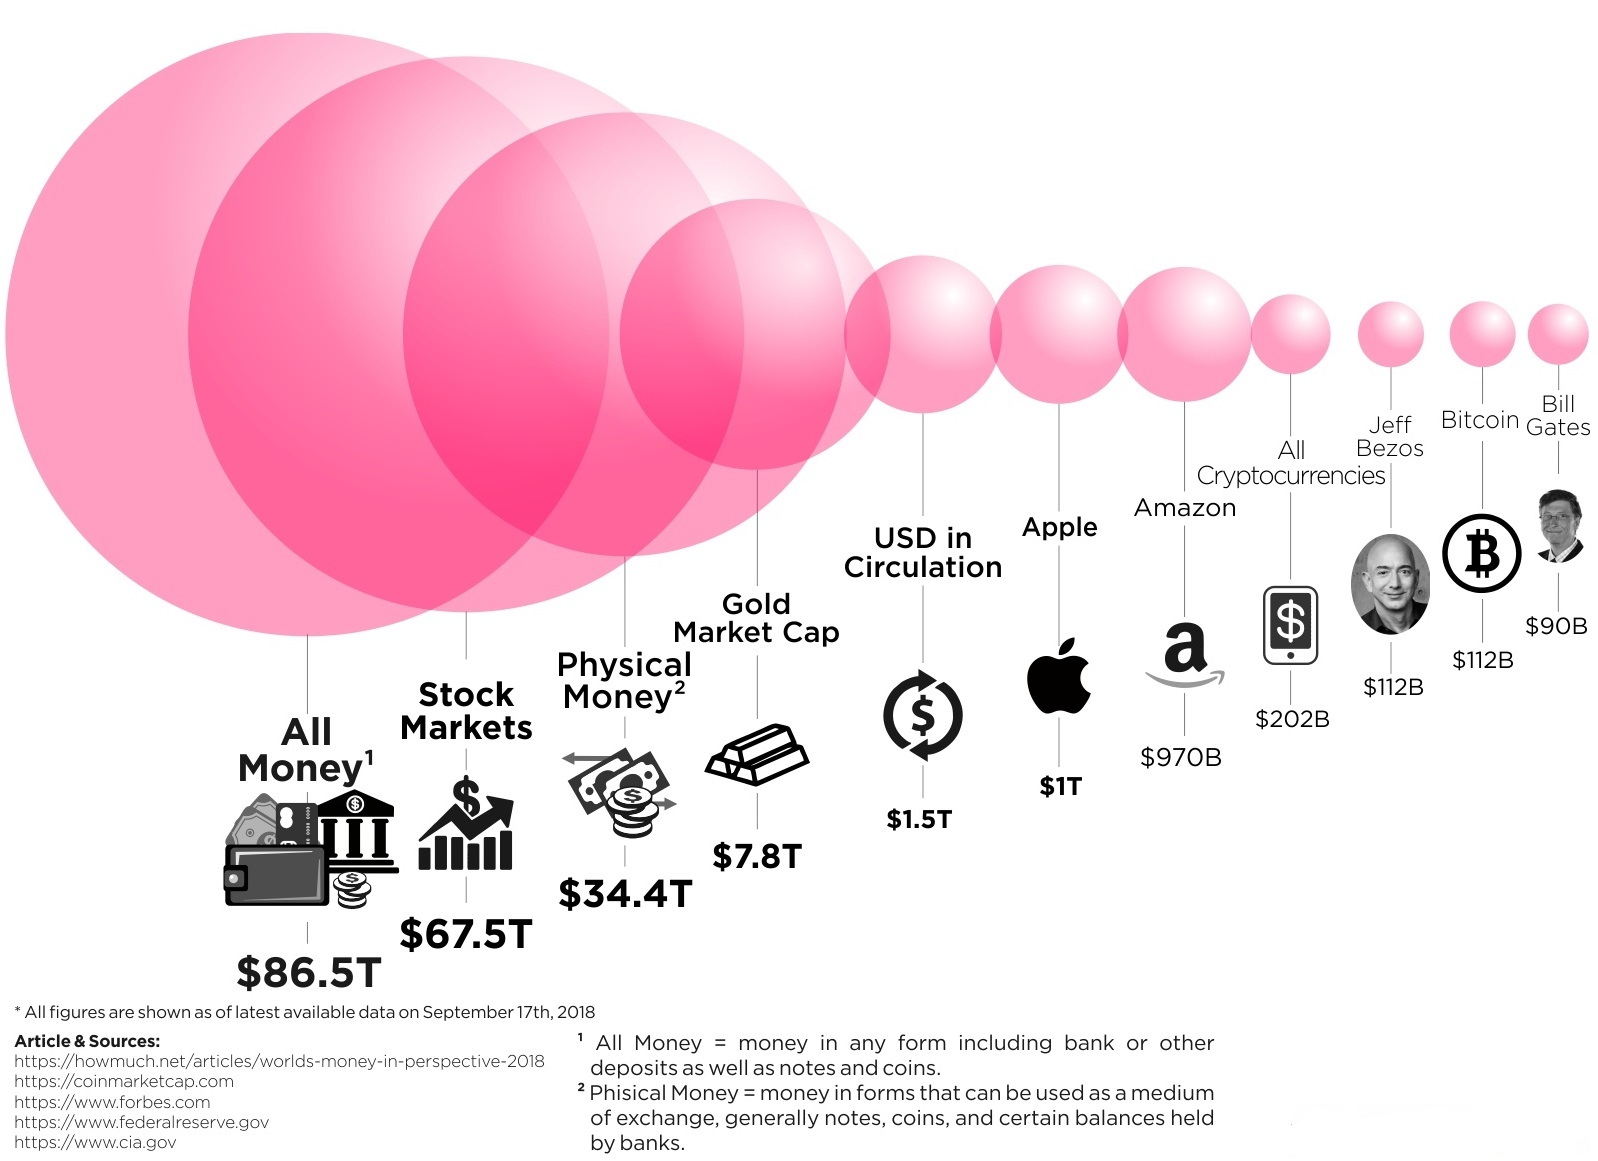
\includegraphics[width=\textwidth]{img/ch-iceage/bitcoin-money-economy-in-perspective-2018.jpg}
    \caption{Cryptocurrency Market in Perspective}
    \label{fig:Cryptocurrency market perspective}
    \source{Howmuch, 2018; \textit{Understanding Money.}}
\end{figure}

\noindent Can you even imagine a billion or a trillion dollars? Cryptocurrencies are a hot topic; not only during the bubble of late 2017/early 2018. However, as soon as the hype was over, the trend reversed. Due to sheer panic, many people sold their assets at terrible losses and are now determined never to touch cryptocurrencies or blockchain technology again, feeling robbed. On the other hand, many people who got in earlier (2013-2017) might have gotten rich quickly. We think that this market is about innovation and change, and the opportunity that comes with it can provide you with disruptive profits.
Furthermore, it is about people and projects using new technology to bring us incredible things. The majority of people in the \say{west} already have access to financial applications, credit and the financial system. As long as nothing drastically impacts their standard of living, there is no immediate sense of urgency and certainly, no specific need to get to know or let alone even use Bitcoin or any other cryptocurrency for that matter.\medskip

What then, about all the people in other areas around the world who don't have easy access to financial services such as banking applications, regular bank accounts, mobile money transfers and the like. Necessity drives adoption, and if there is an urgent requirement, real-world use case and application sprout naturally. Many countries where people don't have access to the financial system are already using new technology to gain access to such services. This technology has the potential to drastically impact and improve the quality of life for many people around the world.\medskip

Although it sounds fantastic, many of these projects still have a very long way to go, which is precisely why this isn't a get-rich-quick scheme for us, but an investment for the (hopefully near) future. Looking at the scale of the different global markets and the stage of blockchain and cryptocurrencies at this point and the problems that are yet to be solved, it is going to take some time for this market to get rid of the volatility and speculation, create liquidity, rid itself of bad actors and get regulated. All of this and more is needed to facilitate the way to mass adoption.

\medskip
\tcbset{colback=orange!3!white,fonttitle=\bfseries}
    \begin{tcolorbox}
    [enhanced,
    title=Bull Market 2017/2018,
    frame style=
    {left color=orange!85!black,right color=yellow!95!black}]
    
               \textit{Speculation and hype were the dominant market forces during the bull market in 2017/2018. Almost every asset was overvalued, and at the same time, the creation of real value was few and far between. Unsustainable and unnatural growth defined this period.}
\end{tcolorbox}

\section{Cryptocurrency Market Compared to S\&P500}
The derivatives markets hold vast amounts (trillions) of dollars and might sound unfamiliar. What about some of the world's biggest companies? Let us have a look at some of the top companies listed in the S\&P500 (Standard \& Poor's 500 Index). The S\&P500 is a market-capitalization-weighted index of the 500 largest U.S. publicly traded companies by market value. The total value of the cryptocurrency market worldwide has come fairly close to the value of a globally recognized corporation such as Apple or Amazon back in January 2018 but has dropped significantly since. Massive volatility is plaguing this emerging market due to a lack of regulation, liquidity and true fundamentals.
Nevertheless, as indicated before, there are close to 6000 projects or cryptocurrencies each of which has its individual and unique goals and ambitions. Some (not all) are utilizing revolutionary new technology and can be very disrupting to existing markets (and thus companies!) in the long run. It might be possible that out of the current 6000 projects - with entrepreneurs around the world launching new projects almost every day - several next-generation companies are bound to emerge.\medskip 

Although the cryptocurrency market might have similarities with big corporations in terms of market share, the point is that many cryptocurrency projects are fundamentally different from regular companies or corporations in the way they operate and function. We highly anticipate at least several successes where blockchain-based projects might have a considerable disruptive impact. In the long term, this will lead to an increase in market share, which is driven by the revolutionary new fundamentals and business models of these new businesses.

\section{Alternative Cryptocurrencies (Altcoins)}
Bitcoin used to dominate the cryptocurrency market prior to the altcoin and ICO boom in 2017. \say{altcoin} is a combination of two words: \say{alt} and \say{coin}; alt signifying \say{alternative} and coin signifying Bitcoin or \say{cryptocurrency}. Together they imply a category of cryptocurrency that is an alternative to the digital cryptocurrency Bitcoin. After the success of Bitcoin, many other peer-to-peer digital cryptocurrencies have emerged in an attempt to imitate that success. 

\medskip
\tcbset{colback=orange!3!white,fonttitle=\bfseries}
    \begin{tcolorbox}
    [enhanced,
    title=Altcoins,
    frame style=
    {left color=orange!85!black,right color=yellow!95!black}]
       \textit{While Bitcoin was the first cryptocurrency, and the only cryptocurrency tested on the biggest scale without any significant failure, it is now only one of more than a thousand cryptocurrencies, which all seek to improve upon Bitcoin or innovate, revolutionize and disrupt in various other segments.}
\end{tcolorbox}
\medskip

Many of these altcoins have built upon the necessary frameworks provided by Bitcoin or have developed their blockchain architecture. Because of the decentralised and distributed architecture of most blockchain networks, most altcoins are peer-to-peer, involving a mining process by which users solve severe problems to unlock blocks and offer efficient and cheap ways to carry out (value) transactions on the web. However, even with many overlapping features, altcoins vary widely from each other - altcoins differentiate themselves from Bitcoin with a range of procedural variations, including different consensus algorithms, transaction speeds and levels of scale-ability. They also deploy various means by which users can mine blocks and get rewarded and make use of application enhancements to - for example - increase user anonymity. As mentioned earlier, there are close to two thousand cryptocurrencies at this time, and that number is growing. Performing fundamental analysis on altcoins is a must before you make any decisions, and we've outlined the basics in our section about doing your research (\cref{ch:research}). Ever since the altcoin explosion in 2017 - Bitcoins dominance has decreased significantly due to ever-increasing numbers of promising projects.

\begin{figure}
    \centering
    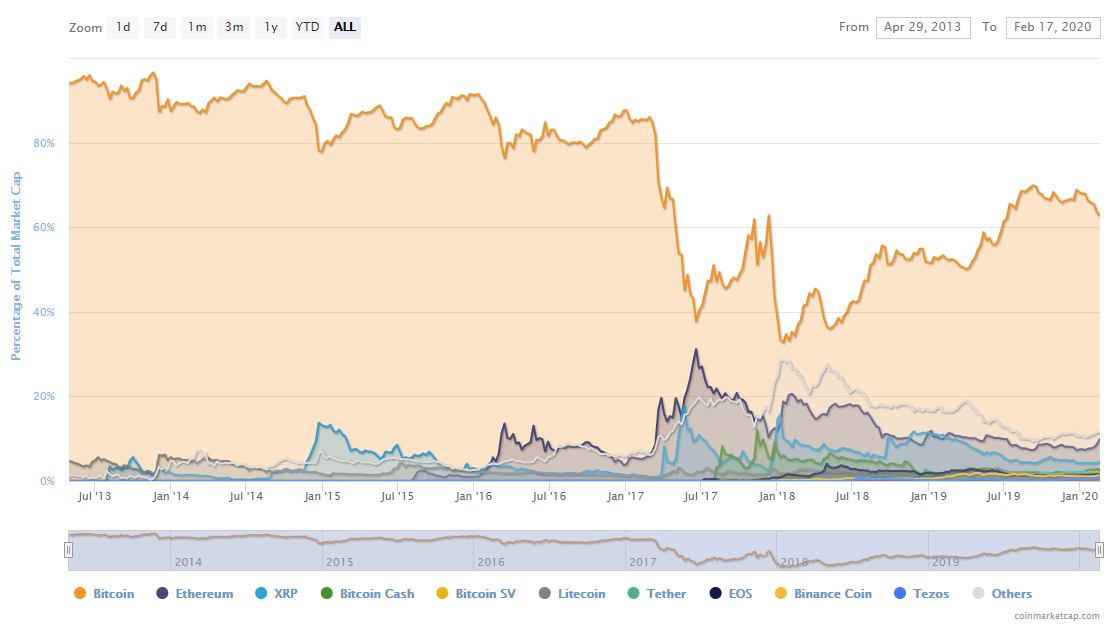
\includegraphics[width=\textwidth]{img/ch-iceage/cmc_domchart_feb2020.PNG}
    \caption{Percentage of the Global Market Cap (Dominance)}
    \label{fig:Total market capitalization dominance}
    \source{Coinmarketcap (17-02-2020); \textit{Global Charts.}}
\end{figure} 

\section{Initial Coin Offerings (ICOs)}
It is incredible to realize how much the altcoin market has grown in the last two years alone. ICOs have become so popular that well over 90\% of total funds raised through this mechanism came from 2018 alone. While it's hard to put this sudden ICO explosion in context, there are animations and info-graphics\footnote{Elementus (39-09-2018); \href{https://elementus.io/blog/ico-market-august-2018}{ICO Market August 2018}.}\footnote{Visual Capitalist (30-12-2017); \href{https://www.visualcapitalist.com/the-rise-of-the-ico}{The Rise of the ICO}.} out there that do the phenomenon sufficient justice by showing a timeline of ICOs and funds raised since early 2014. 

\subsection{ICO scams}

There's a big difference between a typical ICO now and one in 2017. A staggering amount of ICO's didn't even make it to an exchange - according to a study performed on the quality of ICO's by Statis\footnote{Medium (25-05-2018); \href{https://medium.com/satis-group/ico-quality-development-trading-e4fef28df04f}{ICO quality: Development \& Trading}.}. Most of the money is now being raised via private offerings, while public token sales have become rare. Why? Plying retail investors with high-stakes propositions that could (and often do) lose them a ton of money is not a good look. Most ICO projects these days are also taking steps to comply with regulators as almost all ICOs are considered to be securities. Bart Stephens, the co-founder of Blockchain Capital, told The Wall Street Journal that what we are seeing is the \say{normalization} of the ICO market.

Keep in mind that there is always a possibility that a project or a coin is a scam and be skeptical while assessing if it can deliver on what it has promised. People can lose faith, developers can have bad intentions or abandon the project, regulatory policy and compliance frameworks were not even close to being implemented in 2017 (sidelining many institutions), but the regulatory landscape is evolving rapidly. These factors might well have meant the end of your investment if you have invested at the peak of the bubble as prices plummeted and development ground to a standstill. You can check if a coin or project is reported as a scam or a dead coin on Coinopsy\footnote{Coinopsy (05-02-2019);
\href{https://www.coinopsy.com/dead-coins}{Dead Coins}.} and on Deadcoins\footnote{Deadcoins (05-02-2019); \href{https://deadcoins.com}{Full List of Dead Coins}.}. This story has close ties with our section regarding how to perform your research (\cref{ch:research}) and prevent getting scammed. 

